% Created by tikzDevice version 0.12.3.1 on 2023-02-21 12:45:23
% !TEX encoding = UTF-8 Unicode
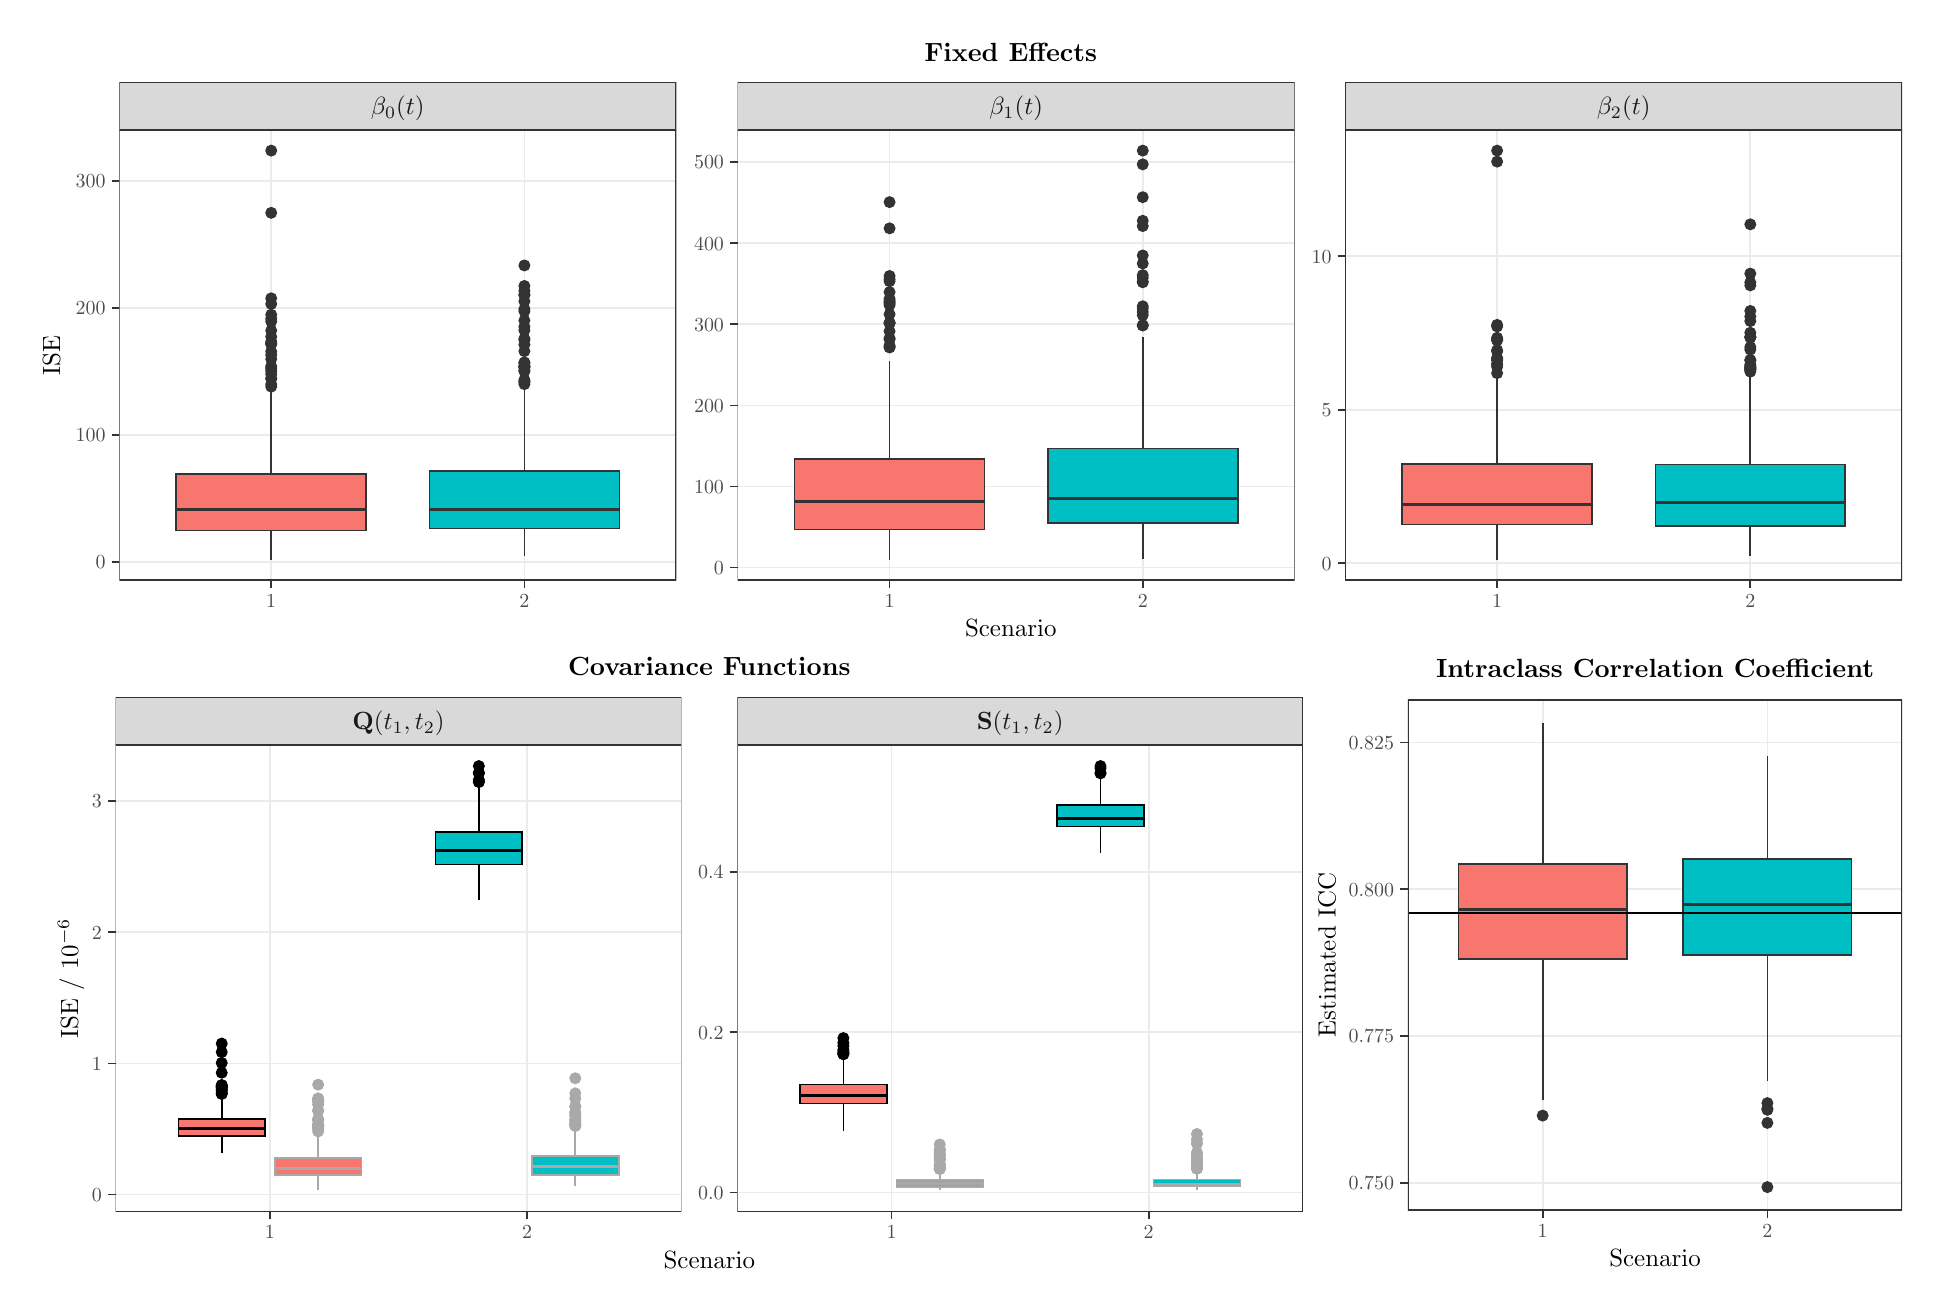
\begin{tikzpicture}[x=1pt,y=1pt]
\definecolor{fillColor}{RGB}{255,255,255}
\path[use as bounding box,fill=fillColor,fill opacity=0.00] (0,0) rectangle (682.86,455.24);
\begin{scope}
\path[clip] (  0.00,227.62) rectangle (682.86,455.24);
\definecolor{drawColor}{RGB}{255,255,255}
\definecolor{fillColor}{RGB}{255,255,255}

\path[draw=drawColor,line width= 0.6pt,line join=round,line cap=round,fill=fillColor] (  0.00,227.62) rectangle (682.86,455.24);
\end{scope}
\begin{scope}
\path[clip] ( 33.11,255.60) rectangle (234.38,418.21);
\definecolor{fillColor}{RGB}{255,255,255}

\path[fill=fillColor] ( 33.11,255.60) rectangle (234.38,418.21);
\definecolor{drawColor}{gray}{0.92}

\path[draw=drawColor,line width= 0.6pt,line join=round] ( 33.11,262.26) --
	(234.38,262.26);

\path[draw=drawColor,line width= 0.6pt,line join=round] ( 33.11,308.12) --
	(234.38,308.12);

\path[draw=drawColor,line width= 0.6pt,line join=round] ( 33.11,353.98) --
	(234.38,353.98);

\path[draw=drawColor,line width= 0.6pt,line join=round] ( 33.11,399.85) --
	(234.38,399.85);

\path[draw=drawColor,line width= 0.6pt,line join=round] ( 88.00,255.60) --
	( 88.00,418.21);

\path[draw=drawColor,line width= 0.6pt,line join=round] (179.49,255.60) --
	(179.49,418.21);
\definecolor{drawColor}{gray}{0.20}
\definecolor{fillColor}{gray}{0.20}

\path[draw=drawColor,line width= 0.4pt,line join=round,line cap=round,fill=fillColor] ( 88.00,341.16) circle (  1.96);

\path[draw=drawColor,line width= 0.4pt,line join=round,line cap=round,fill=fillColor] ( 88.00,351.52) circle (  1.96);

\path[draw=drawColor,line width= 0.4pt,line join=round,line cap=round,fill=fillColor] ( 88.00,328.55) circle (  1.96);

\path[draw=drawColor,line width= 0.4pt,line join=round,line cap=round,fill=fillColor] ( 88.00,357.44) circle (  1.96);

\path[draw=drawColor,line width= 0.4pt,line join=round,line cap=round,fill=fillColor] ( 88.00,332.32) circle (  1.96);

\path[draw=drawColor,line width= 0.4pt,line join=round,line cap=round,fill=fillColor] ( 88.00,349.05) circle (  1.96);

\path[draw=drawColor,line width= 0.4pt,line join=round,line cap=round,fill=fillColor] ( 88.00,345.80) circle (  1.96);

\path[draw=drawColor,line width= 0.4pt,line join=round,line cap=round,fill=fillColor] ( 88.00,340.93) circle (  1.96);

\path[draw=drawColor,line width= 0.4pt,line join=round,line cap=round,fill=fillColor] ( 88.00,338.26) circle (  1.96);

\path[draw=drawColor,line width= 0.4pt,line join=round,line cap=round,fill=fillColor] ( 88.00,336.95) circle (  1.96);

\path[draw=drawColor,line width= 0.4pt,line join=round,line cap=round,fill=fillColor] ( 88.00,328.36) circle (  1.96);

\path[draw=drawColor,line width= 0.4pt,line join=round,line cap=round,fill=fillColor] ( 88.00,325.53) circle (  1.96);

\path[draw=drawColor,line width= 0.4pt,line join=round,line cap=round,fill=fillColor] ( 88.00,350.13) circle (  1.96);

\path[draw=drawColor,line width= 0.4pt,line join=round,line cap=round,fill=fillColor] ( 88.00,410.81) circle (  1.96);

\path[draw=drawColor,line width= 0.4pt,line join=round,line cap=round,fill=fillColor] ( 88.00,330.01) circle (  1.96);

\path[draw=drawColor,line width= 0.4pt,line join=round,line cap=round,fill=fillColor] ( 88.00,335.50) circle (  1.96);

\path[draw=drawColor,line width= 0.4pt,line join=round,line cap=round,fill=fillColor] ( 88.00,331.87) circle (  1.96);

\path[draw=drawColor,line width= 0.4pt,line join=round,line cap=round,fill=fillColor] ( 88.00,343.57) circle (  1.96);

\path[draw=drawColor,line width= 0.4pt,line join=round,line cap=round,fill=fillColor] ( 88.00,331.05) circle (  1.96);

\path[draw=drawColor,line width= 0.4pt,line join=round,line cap=round,fill=fillColor] ( 88.00,388.33) circle (  1.96);

\path[draw=drawColor,line width= 0.4pt,line join=round,line cap=round,fill=fillColor] ( 88.00,332.92) circle (  1.96);

\path[draw=drawColor,line width= 0.4pt,line join=round,line cap=round,fill=fillColor] ( 88.00,340.93) circle (  1.96);

\path[draw=drawColor,line width= 0.4pt,line join=round,line cap=round,fill=fillColor] ( 88.00,326.35) circle (  1.96);

\path[draw=drawColor,line width= 0.4pt,line join=round,line cap=round,fill=fillColor] ( 88.00,341.83) circle (  1.96);

\path[draw=drawColor,line width= 0.4pt,line join=round,line cap=round,fill=fillColor] ( 88.00,355.42) circle (  1.96);

\path[draw=drawColor,line width= 0.6pt,line join=round] ( 88.00,294.03) -- ( 88.00,324.57);

\path[draw=drawColor,line width= 0.6pt,line join=round] ( 88.00,273.50) -- ( 88.00,262.99);
\definecolor{fillColor}{RGB}{248,118,109}

\path[draw=drawColor,line width= 0.6pt,fill=fillColor] ( 53.69,294.03) --
	( 53.69,273.50) --
	(122.31,273.50) --
	(122.31,294.03) --
	( 53.69,294.03) --
	cycle;

\path[draw=drawColor,line width= 1.1pt] ( 53.69,281.27) -- (122.31,281.27);
\definecolor{fillColor}{gray}{0.20}

\path[draw=drawColor,line width= 0.4pt,line join=round,line cap=round,fill=fillColor] (179.49,353.58) circle (  1.96);

\path[draw=drawColor,line width= 0.4pt,line join=round,line cap=round,fill=fillColor] (179.49,328.00) circle (  1.96);

\path[draw=drawColor,line width= 0.4pt,line join=round,line cap=round,fill=fillColor] (179.49,332.66) circle (  1.96);

\path[draw=drawColor,line width= 0.4pt,line join=round,line cap=round,fill=fillColor] (179.49,331.07) circle (  1.96);

\path[draw=drawColor,line width= 0.4pt,line join=round,line cap=round,fill=fillColor] (179.49,334.29) circle (  1.96);

\path[draw=drawColor,line width= 0.4pt,line join=round,line cap=round,fill=fillColor] (179.49,358.57) circle (  1.96);

\path[draw=drawColor,line width= 0.4pt,line join=round,line cap=round,fill=fillColor] (179.49,340.72) circle (  1.96);

\path[draw=drawColor,line width= 0.4pt,line join=round,line cap=round,fill=fillColor] (179.49,331.36) circle (  1.96);

\path[draw=drawColor,line width= 0.4pt,line join=round,line cap=round,fill=fillColor] (179.49,360.15) circle (  1.96);

\path[draw=drawColor,line width= 0.4pt,line join=round,line cap=round,fill=fillColor] (179.49,332.30) circle (  1.96);

\path[draw=drawColor,line width= 0.4pt,line join=round,line cap=round,fill=fillColor] (179.49,333.99) circle (  1.96);

\path[draw=drawColor,line width= 0.4pt,line join=round,line cap=round,fill=fillColor] (179.49,327.23) circle (  1.96);

\path[draw=drawColor,line width= 0.4pt,line join=round,line cap=round,fill=fillColor] (179.49,349.46) circle (  1.96);

\path[draw=drawColor,line width= 0.4pt,line join=round,line cap=round,fill=fillColor] (179.49,358.74) circle (  1.96);

\path[draw=drawColor,line width= 0.4pt,line join=round,line cap=round,fill=fillColor] (179.49,352.75) circle (  1.96);

\path[draw=drawColor,line width= 0.4pt,line join=round,line cap=round,fill=fillColor] (179.49,342.86) circle (  1.96);

\path[draw=drawColor,line width= 0.4pt,line join=round,line cap=round,fill=fillColor] (179.49,356.37) circle (  1.96);

\path[draw=drawColor,line width= 0.4pt,line join=round,line cap=round,fill=fillColor] (179.49,338.34) circle (  1.96);

\path[draw=drawColor,line width= 0.4pt,line join=round,line cap=round,fill=fillColor] (179.49,327.32) circle (  1.96);

\path[draw=drawColor,line width= 0.4pt,line join=round,line cap=round,fill=fillColor] (179.49,332.80) circle (  1.96);

\path[draw=drawColor,line width= 0.4pt,line join=round,line cap=round,fill=fillColor] (179.49,326.43) circle (  1.96);

\path[draw=drawColor,line width= 0.4pt,line join=round,line cap=round,fill=fillColor] (179.49,333.04) circle (  1.96);

\path[draw=drawColor,line width= 0.4pt,line join=round,line cap=round,fill=fillColor] (179.49,361.91) circle (  1.96);

\path[draw=drawColor,line width= 0.4pt,line join=round,line cap=round,fill=fillColor] (179.49,369.32) circle (  1.96);

\path[draw=drawColor,line width= 0.4pt,line join=round,line cap=round,fill=fillColor] (179.49,345.88) circle (  1.96);

\path[draw=drawColor,line width= 0.4pt,line join=round,line cap=round,fill=fillColor] (179.49,347.18) circle (  1.96);

\path[draw=drawColor,line width= 0.4pt,line join=round,line cap=round,fill=fillColor] (179.49,342.37) circle (  1.96);

\path[draw=drawColor,line width= 0.6pt,line join=round] (179.49,295.01) -- (179.49,324.23);

\path[draw=drawColor,line width= 0.6pt,line join=round] (179.49,274.28) -- (179.49,264.41);
\definecolor{fillColor}{RGB}{0,191,196}

\path[draw=drawColor,line width= 0.6pt,fill=fillColor] (145.18,295.01) --
	(145.18,274.28) --
	(213.80,274.28) --
	(213.80,295.01) --
	(145.18,295.01) --
	cycle;

\path[draw=drawColor,line width= 1.1pt] (145.18,281.06) -- (213.80,281.06);

\path[draw=drawColor,line width= 0.6pt,line join=round,line cap=round] ( 33.11,255.60) rectangle (234.38,418.21);
\end{scope}
\begin{scope}
\path[clip] (256.55,255.60) rectangle (457.83,418.21);
\definecolor{fillColor}{RGB}{255,255,255}

\path[fill=fillColor] (256.55,255.60) rectangle (457.83,418.21);
\definecolor{drawColor}{gray}{0.92}

\path[draw=drawColor,line width= 0.6pt,line join=round] (256.55,260.15) --
	(457.83,260.15);

\path[draw=drawColor,line width= 0.6pt,line join=round] (256.55,289.46) --
	(457.83,289.46);

\path[draw=drawColor,line width= 0.6pt,line join=round] (256.55,318.76) --
	(457.83,318.76);

\path[draw=drawColor,line width= 0.6pt,line join=round] (256.55,348.07) --
	(457.83,348.07);

\path[draw=drawColor,line width= 0.6pt,line join=round] (256.55,377.37) --
	(457.83,377.37);

\path[draw=drawColor,line width= 0.6pt,line join=round] (256.55,406.68) --
	(457.83,406.68);

\path[draw=drawColor,line width= 0.6pt,line join=round] (311.44,255.60) --
	(311.44,418.21);

\path[draw=drawColor,line width= 0.6pt,line join=round] (402.93,255.60) --
	(402.93,418.21);
\definecolor{drawColor}{gray}{0.20}
\definecolor{fillColor}{gray}{0.20}

\path[draw=drawColor,line width= 0.4pt,line join=round,line cap=round,fill=fillColor] (311.44,339.83) circle (  1.96);

\path[draw=drawColor,line width= 0.4pt,line join=round,line cap=round,fill=fillColor] (311.44,364.39) circle (  1.96);

\path[draw=drawColor,line width= 0.4pt,line join=round,line cap=round,fill=fillColor] (311.44,382.73) circle (  1.96);

\path[draw=drawColor,line width= 0.4pt,line join=round,line cap=round,fill=fillColor] (311.44,392.20) circle (  1.96);

\path[draw=drawColor,line width= 0.4pt,line join=round,line cap=round,fill=fillColor] (311.44,356.54) circle (  1.96);

\path[draw=drawColor,line width= 0.4pt,line join=round,line cap=round,fill=fillColor] (311.44,342.62) circle (  1.96);

\path[draw=drawColor,line width= 0.4pt,line join=round,line cap=round,fill=fillColor] (311.44,365.51) circle (  1.96);

\path[draw=drawColor,line width= 0.4pt,line join=round,line cap=round,fill=fillColor] (311.44,343.05) circle (  1.96);

\path[draw=drawColor,line width= 0.4pt,line join=round,line cap=round,fill=fillColor] (311.44,348.60) circle (  1.96);

\path[draw=drawColor,line width= 0.4pt,line join=round,line cap=round,fill=fillColor] (311.44,359.69) circle (  1.96);

\path[draw=drawColor,line width= 0.4pt,line join=round,line cap=round,fill=fillColor] (311.44,348.51) circle (  1.96);

\path[draw=drawColor,line width= 0.4pt,line join=round,line cap=round,fill=fillColor] (311.44,354.95) circle (  1.96);

\path[draw=drawColor,line width= 0.4pt,line join=round,line cap=round,fill=fillColor] (311.44,340.44) circle (  1.96);

\path[draw=drawColor,line width= 0.4pt,line join=round,line cap=round,fill=fillColor] (311.44,345.55) circle (  1.96);

\path[draw=drawColor,line width= 0.4pt,line join=round,line cap=round,fill=fillColor] (311.44,355.63) circle (  1.96);

\path[draw=drawColor,line width= 0.4pt,line join=round,line cap=round,fill=fillColor] (311.44,348.51) circle (  1.96);

\path[draw=drawColor,line width= 0.4pt,line join=round,line cap=round,fill=fillColor] (311.44,356.06) circle (  1.96);

\path[draw=drawColor,line width= 0.4pt,line join=round,line cap=round,fill=fillColor] (311.44,363.61) circle (  1.96);

\path[draw=drawColor,line width= 0.4pt,line join=round,line cap=round,fill=fillColor] (311.44,357.29) circle (  1.96);

\path[draw=drawColor,line width= 0.4pt,line join=round,line cap=round,fill=fillColor] (311.44,351.68) circle (  1.96);

\path[draw=drawColor,line width= 0.4pt,line join=round,line cap=round,fill=fillColor] (311.44,339.68) circle (  1.96);

\path[draw=drawColor,line width= 0.6pt,line join=round] (311.44,299.46) -- (311.44,334.71);

\path[draw=drawColor,line width= 0.6pt,line join=round] (311.44,273.93) -- (311.44,262.99);
\definecolor{fillColor}{RGB}{248,118,109}

\path[draw=drawColor,line width= 0.6pt,fill=fillColor] (277.14,299.46) --
	(277.14,273.93) --
	(345.75,273.93) --
	(345.75,299.46) --
	(277.14,299.46) --
	cycle;

\path[draw=drawColor,line width= 1.1pt] (277.14,283.97) -- (345.75,283.97);
\definecolor{fillColor}{gray}{0.20}

\path[draw=drawColor,line width= 0.4pt,line join=round,line cap=round,fill=fillColor] (402.93,353.75) circle (  1.96);

\path[draw=drawColor,line width= 0.4pt,line join=round,line cap=round,fill=fillColor] (402.93,370.03) circle (  1.96);

\path[draw=drawColor,line width= 0.4pt,line join=round,line cap=round,fill=fillColor] (402.93,365.82) circle (  1.96);

\path[draw=drawColor,line width= 0.4pt,line join=round,line cap=round,fill=fillColor] (402.93,352.53) circle (  1.96);

\path[draw=drawColor,line width= 0.4pt,line join=round,line cap=round,fill=fillColor] (402.93,354.57) circle (  1.96);

\path[draw=drawColor,line width= 0.4pt,line join=round,line cap=round,fill=fillColor] (402.93,363.23) circle (  1.96);

\path[draw=drawColor,line width= 0.4pt,line join=round,line cap=round,fill=fillColor] (402.93,383.54) circle (  1.96);

\path[draw=drawColor,line width= 0.4pt,line join=round,line cap=round,fill=fillColor] (402.93,363.46) circle (  1.96);

\path[draw=drawColor,line width= 0.4pt,line join=round,line cap=round,fill=fillColor] (402.93,351.36) circle (  1.96);

\path[draw=drawColor,line width= 0.4pt,line join=round,line cap=round,fill=fillColor] (402.93,347.62) circle (  1.96);

\path[draw=drawColor,line width= 0.4pt,line join=round,line cap=round,fill=fillColor] (402.93,364.84) circle (  1.96);

\path[draw=drawColor,line width= 0.4pt,line join=round,line cap=round,fill=fillColor] (402.93,393.98) circle (  1.96);

\path[draw=drawColor,line width= 0.4pt,line join=round,line cap=round,fill=fillColor] (402.93,372.93) circle (  1.96);

\path[draw=drawColor,line width= 0.4pt,line join=round,line cap=round,fill=fillColor] (402.93,405.85) circle (  1.96);

\path[draw=drawColor,line width= 0.4pt,line join=round,line cap=round,fill=fillColor] (402.93,410.81) circle (  1.96);

\path[draw=drawColor,line width= 0.4pt,line join=round,line cap=round,fill=fillColor] (402.93,385.45) circle (  1.96);

\path[draw=drawColor,line width= 0.4pt,line join=round,line cap=round,fill=fillColor] (402.93,347.71) circle (  1.96);

\path[draw=drawColor,line width= 0.6pt,line join=round] (402.93,303.18) -- (402.93,343.55);

\path[draw=drawColor,line width= 0.6pt,line join=round] (402.93,276.20) -- (402.93,263.30);
\definecolor{fillColor}{RGB}{0,191,196}

\path[draw=drawColor,line width= 0.6pt,fill=fillColor] (368.62,303.18) --
	(368.62,276.20) --
	(437.24,276.20) --
	(437.24,303.18) --
	(368.62,303.18) --
	cycle;

\path[draw=drawColor,line width= 1.1pt] (368.62,285.13) -- (437.24,285.13);

\path[draw=drawColor,line width= 0.6pt,line join=round,line cap=round] (256.55,255.60) rectangle (457.83,418.21);
\end{scope}
\begin{scope}
\path[clip] (476.09,255.60) rectangle (677.36,418.21);
\definecolor{fillColor}{RGB}{255,255,255}

\path[fill=fillColor] (476.09,255.60) rectangle (677.36,418.21);
\definecolor{drawColor}{gray}{0.92}

\path[draw=drawColor,line width= 0.6pt,line join=round] (476.09,261.74) --
	(677.36,261.74);

\path[draw=drawColor,line width= 0.6pt,line join=round] (476.09,317.18) --
	(677.36,317.18);

\path[draw=drawColor,line width= 0.6pt,line join=round] (476.09,372.62) --
	(677.36,372.62);

\path[draw=drawColor,line width= 0.6pt,line join=round] (530.98,255.60) --
	(530.98,418.21);

\path[draw=drawColor,line width= 0.6pt,line join=round] (622.47,255.60) --
	(622.47,418.21);
\definecolor{drawColor}{gray}{0.20}
\definecolor{fillColor}{gray}{0.20}

\path[draw=drawColor,line width= 0.4pt,line join=round,line cap=round,fill=fillColor] (530.98,347.85) circle (  1.96);

\path[draw=drawColor,line width= 0.4pt,line join=round,line cap=round,fill=fillColor] (530.98,338.72) circle (  1.96);

\path[draw=drawColor,line width= 0.4pt,line join=round,line cap=round,fill=fillColor] (530.98,332.71) circle (  1.96);

\path[draw=drawColor,line width= 0.4pt,line join=round,line cap=round,fill=fillColor] (530.98,330.40) circle (  1.96);

\path[draw=drawColor,line width= 0.4pt,line join=round,line cap=round,fill=fillColor] (530.98,347.26) circle (  1.96);

\path[draw=drawColor,line width= 0.4pt,line join=round,line cap=round,fill=fillColor] (530.98,343.17) circle (  1.96);

\path[draw=drawColor,line width= 0.4pt,line join=round,line cap=round,fill=fillColor] (530.98,410.81) circle (  1.96);

\path[draw=drawColor,line width= 0.4pt,line join=round,line cap=round,fill=fillColor] (530.98,335.73) circle (  1.96);

\path[draw=drawColor,line width= 0.4pt,line join=round,line cap=round,fill=fillColor] (530.98,335.85) circle (  1.96);

\path[draw=drawColor,line width= 0.4pt,line join=round,line cap=round,fill=fillColor] (530.98,406.83) circle (  1.96);

\path[draw=drawColor,line width= 0.4pt,line join=round,line cap=round,fill=fillColor] (530.98,333.71) circle (  1.96);

\path[draw=drawColor,line width= 0.4pt,line join=round,line cap=round,fill=fillColor] (530.98,333.65) circle (  1.96);

\path[draw=drawColor,line width= 0.4pt,line join=round,line cap=round,fill=fillColor] (530.98,342.45) circle (  1.96);

\path[draw=drawColor,line width= 0.4pt,line join=round,line cap=round,fill=fillColor] (530.98,335.13) circle (  1.96);

\path[draw=drawColor,line width= 0.4pt,line join=round,line cap=round,fill=fillColor] (530.98,335.17) circle (  1.96);

\path[draw=drawColor,line width= 0.4pt,line join=round,line cap=round,fill=fillColor] (530.98,338.27) circle (  1.96);

\path[draw=drawColor,line width= 0.4pt,line join=round,line cap=round,fill=fillColor] (530.98,342.50) circle (  1.96);

\path[draw=drawColor,line width= 0.4pt,line join=round,line cap=round,fill=fillColor] (530.98,342.29) circle (  1.96);

\path[draw=drawColor,line width= 0.6pt,line join=round] (530.98,297.49) -- (530.98,329.17);

\path[draw=drawColor,line width= 0.6pt,line join=round] (530.98,275.69) -- (530.98,262.99);
\definecolor{fillColor}{RGB}{248,118,109}

\path[draw=drawColor,line width= 0.6pt,fill=fillColor] (496.67,297.49) --
	(496.67,275.69) --
	(565.29,275.69) --
	(565.29,297.49) --
	(496.67,297.49) --
	cycle;

\path[draw=drawColor,line width= 1.1pt] (496.67,282.79) -- (565.29,282.79);
\definecolor{fillColor}{gray}{0.20}

\path[draw=drawColor,line width= 0.4pt,line join=round,line cap=round,fill=fillColor] (622.47,343.37) circle (  1.96);

\path[draw=drawColor,line width= 0.4pt,line join=round,line cap=round,fill=fillColor] (622.47,338.91) circle (  1.96);

\path[draw=drawColor,line width= 0.4pt,line join=round,line cap=round,fill=fillColor] (622.47,345.00) circle (  1.96);

\path[draw=drawColor,line width= 0.4pt,line join=round,line cap=round,fill=fillColor] (622.47,331.66) circle (  1.96);

\path[draw=drawColor,line width= 0.4pt,line join=round,line cap=round,fill=fillColor] (622.47,335.01) circle (  1.96);

\path[draw=drawColor,line width= 0.4pt,line join=round,line cap=round,fill=fillColor] (622.47,366.37) circle (  1.96);

\path[draw=drawColor,line width= 0.4pt,line join=round,line cap=round,fill=fillColor] (622.47,331.70) circle (  1.96);

\path[draw=drawColor,line width= 0.4pt,line join=round,line cap=round,fill=fillColor] (622.47,332.42) circle (  1.96);

\path[draw=drawColor,line width= 0.4pt,line join=round,line cap=round,fill=fillColor] (622.47,362.12) circle (  1.96);

\path[draw=drawColor,line width= 0.4pt,line join=round,line cap=round,fill=fillColor] (622.47,343.33) circle (  1.96);

\path[draw=drawColor,line width= 0.4pt,line join=round,line cap=round,fill=fillColor] (622.47,384.17) circle (  1.96);

\path[draw=drawColor,line width= 0.4pt,line join=round,line cap=round,fill=fillColor] (622.47,349.21) circle (  1.96);

\path[draw=drawColor,line width= 0.4pt,line join=round,line cap=round,fill=fillColor] (622.47,343.51) circle (  1.96);

\path[draw=drawColor,line width= 0.4pt,line join=round,line cap=round,fill=fillColor] (622.47,335.16) circle (  1.96);

\path[draw=drawColor,line width= 0.4pt,line join=round,line cap=round,fill=fillColor] (622.47,332.88) circle (  1.96);

\path[draw=drawColor,line width= 0.4pt,line join=round,line cap=round,fill=fillColor] (622.47,339.84) circle (  1.96);

\path[draw=drawColor,line width= 0.4pt,line join=round,line cap=round,fill=fillColor] (622.47,363.19) circle (  1.96);

\path[draw=drawColor,line width= 0.4pt,line join=round,line cap=round,fill=fillColor] (622.47,332.64) circle (  1.96);

\path[draw=drawColor,line width= 0.4pt,line join=round,line cap=round,fill=fillColor] (622.47,332.03) circle (  1.96);

\path[draw=drawColor,line width= 0.4pt,line join=round,line cap=round,fill=fillColor] (622.47,330.94) circle (  1.96);

\path[draw=drawColor,line width= 0.4pt,line join=round,line cap=round,fill=fillColor] (622.47,350.86) circle (  1.96);

\path[draw=drawColor,line width= 0.4pt,line join=round,line cap=round,fill=fillColor] (622.47,352.88) circle (  1.96);

\path[draw=drawColor,line width= 0.4pt,line join=round,line cap=round,fill=fillColor] (622.47,331.78) circle (  1.96);

\path[draw=drawColor,line width= 0.4pt,line join=round,line cap=round,fill=fillColor] (622.47,333.50) circle (  1.96);

\path[draw=drawColor,line width= 0.6pt,line join=round] (622.47,297.40) -- (622.47,330.50);

\path[draw=drawColor,line width= 0.6pt,line join=round] (622.47,275.17) -- (622.47,264.48);
\definecolor{fillColor}{RGB}{0,191,196}

\path[draw=drawColor,line width= 0.6pt,fill=fillColor] (588.16,297.40) --
	(588.16,275.17) --
	(656.78,275.17) --
	(656.78,297.40) --
	(588.16,297.40) --
	cycle;

\path[draw=drawColor,line width= 1.1pt] (588.16,283.73) -- (656.78,283.73);

\path[draw=drawColor,line width= 0.6pt,line join=round,line cap=round] (476.09,255.60) rectangle (677.36,418.21);
\end{scope}
\begin{scope}
\path[clip] ( 33.11,418.21) rectangle (234.38,435.48);
\definecolor{drawColor}{gray}{0.20}
\definecolor{fillColor}{gray}{0.85}

\path[draw=drawColor,line width= 0.6pt,line join=round,line cap=round,fill=fillColor] ( 33.11,418.21) rectangle (234.38,435.48);
\definecolor{drawColor}{gray}{0.10}

\node[text=drawColor,anchor=base,inner sep=0pt, outer sep=0pt, scale=  0.90] at (133.74,423.74) {$\boldsymbol{\beta}_0(t)$};
\end{scope}
\begin{scope}
\path[clip] (256.55,418.21) rectangle (457.83,435.48);
\definecolor{drawColor}{gray}{0.20}
\definecolor{fillColor}{gray}{0.85}

\path[draw=drawColor,line width= 0.6pt,line join=round,line cap=round,fill=fillColor] (256.55,418.21) rectangle (457.83,435.48);
\definecolor{drawColor}{gray}{0.10}

\node[text=drawColor,anchor=base,inner sep=0pt, outer sep=0pt, scale=  0.90] at (357.19,423.74) {$\boldsymbol{\beta}_1 (t)$};
\end{scope}
\begin{scope}
\path[clip] (476.09,418.21) rectangle (677.36,435.48);
\definecolor{drawColor}{gray}{0.20}
\definecolor{fillColor}{gray}{0.85}

\path[draw=drawColor,line width= 0.6pt,line join=round,line cap=round,fill=fillColor] (476.09,418.21) rectangle (677.36,435.48);
\definecolor{drawColor}{gray}{0.10}

\node[text=drawColor,anchor=base,inner sep=0pt, outer sep=0pt, scale=  0.90] at (576.73,423.74) {$\boldsymbol{\beta}_2 (t)$};
\end{scope}
\begin{scope}
\path[clip] (  0.00,  0.00) rectangle (682.86,455.24);
\definecolor{drawColor}{gray}{0.20}

\path[draw=drawColor,line width= 0.6pt,line join=round] ( 88.00,252.85) --
	( 88.00,255.60);

\path[draw=drawColor,line width= 0.6pt,line join=round] (179.49,252.85) --
	(179.49,255.60);
\end{scope}
\begin{scope}
\path[clip] (  0.00,  0.00) rectangle (682.86,455.24);
\definecolor{drawColor}{gray}{0.30}

\node[text=drawColor,anchor=base,inner sep=0pt, outer sep=0pt, scale=  0.72] at ( 88.00,245.69) {1};

\node[text=drawColor,anchor=base,inner sep=0pt, outer sep=0pt, scale=  0.72] at (179.49,245.69) {2};
\end{scope}
\begin{scope}
\path[clip] (  0.00,  0.00) rectangle (682.86,455.24);
\definecolor{drawColor}{gray}{0.20}

\path[draw=drawColor,line width= 0.6pt,line join=round] (311.44,252.85) --
	(311.44,255.60);

\path[draw=drawColor,line width= 0.6pt,line join=round] (402.93,252.85) --
	(402.93,255.60);
\end{scope}
\begin{scope}
\path[clip] (  0.00,  0.00) rectangle (682.86,455.24);
\definecolor{drawColor}{gray}{0.30}

\node[text=drawColor,anchor=base,inner sep=0pt, outer sep=0pt, scale=  0.72] at (311.44,245.69) {1};

\node[text=drawColor,anchor=base,inner sep=0pt, outer sep=0pt, scale=  0.72] at (402.93,245.69) {2};
\end{scope}
\begin{scope}
\path[clip] (  0.00,  0.00) rectangle (682.86,455.24);
\definecolor{drawColor}{gray}{0.20}

\path[draw=drawColor,line width= 0.6pt,line join=round] (530.98,252.85) --
	(530.98,255.60);

\path[draw=drawColor,line width= 0.6pt,line join=round] (622.47,252.85) --
	(622.47,255.60);
\end{scope}
\begin{scope}
\path[clip] (  0.00,  0.00) rectangle (682.86,455.24);
\definecolor{drawColor}{gray}{0.30}

\node[text=drawColor,anchor=base,inner sep=0pt, outer sep=0pt, scale=  0.72] at (530.98,245.69) {1};

\node[text=drawColor,anchor=base,inner sep=0pt, outer sep=0pt, scale=  0.72] at (622.47,245.69) {2};
\end{scope}
\begin{scope}
\path[clip] (  0.00,  0.00) rectangle (682.86,455.24);
\definecolor{drawColor}{gray}{0.30}

\node[text=drawColor,anchor=base east,inner sep=0pt, outer sep=0pt, scale=  0.72] at (471.14,259.26) {0};

\node[text=drawColor,anchor=base east,inner sep=0pt, outer sep=0pt, scale=  0.72] at (471.14,314.70) {5};

\node[text=drawColor,anchor=base east,inner sep=0pt, outer sep=0pt, scale=  0.72] at (471.14,370.15) {10};
\end{scope}
\begin{scope}
\path[clip] (  0.00,  0.00) rectangle (682.86,455.24);
\definecolor{drawColor}{gray}{0.20}

\path[draw=drawColor,line width= 0.6pt,line join=round] (473.34,261.74) --
	(476.09,261.74);

\path[draw=drawColor,line width= 0.6pt,line join=round] (473.34,317.18) --
	(476.09,317.18);

\path[draw=drawColor,line width= 0.6pt,line join=round] (473.34,372.62) --
	(476.09,372.62);
\end{scope}
\begin{scope}
\path[clip] (  0.00,  0.00) rectangle (682.86,455.24);
\definecolor{drawColor}{gray}{0.30}

\node[text=drawColor,anchor=base east,inner sep=0pt, outer sep=0pt, scale=  0.72] at (251.60,257.67) {0};

\node[text=drawColor,anchor=base east,inner sep=0pt, outer sep=0pt, scale=  0.72] at (251.60,286.98) {100};

\node[text=drawColor,anchor=base east,inner sep=0pt, outer sep=0pt, scale=  0.72] at (251.60,316.28) {200};

\node[text=drawColor,anchor=base east,inner sep=0pt, outer sep=0pt, scale=  0.72] at (251.60,345.59) {300};

\node[text=drawColor,anchor=base east,inner sep=0pt, outer sep=0pt, scale=  0.72] at (251.60,374.89) {400};

\node[text=drawColor,anchor=base east,inner sep=0pt, outer sep=0pt, scale=  0.72] at (251.60,404.20) {500};
\end{scope}
\begin{scope}
\path[clip] (  0.00,  0.00) rectangle (682.86,455.24);
\definecolor{drawColor}{gray}{0.20}

\path[draw=drawColor,line width= 0.6pt,line join=round] (253.80,260.15) --
	(256.55,260.15);

\path[draw=drawColor,line width= 0.6pt,line join=round] (253.80,289.46) --
	(256.55,289.46);

\path[draw=drawColor,line width= 0.6pt,line join=round] (253.80,318.76) --
	(256.55,318.76);

\path[draw=drawColor,line width= 0.6pt,line join=round] (253.80,348.07) --
	(256.55,348.07);

\path[draw=drawColor,line width= 0.6pt,line join=round] (253.80,377.37) --
	(256.55,377.37);

\path[draw=drawColor,line width= 0.6pt,line join=round] (253.80,406.68) --
	(256.55,406.68);
\end{scope}
\begin{scope}
\path[clip] (  0.00,  0.00) rectangle (682.86,455.24);
\definecolor{drawColor}{gray}{0.30}

\node[text=drawColor,anchor=base east,inner sep=0pt, outer sep=0pt, scale=  0.72] at ( 28.16,259.78) {0};

\node[text=drawColor,anchor=base east,inner sep=0pt, outer sep=0pt, scale=  0.72] at ( 28.16,305.64) {100};

\node[text=drawColor,anchor=base east,inner sep=0pt, outer sep=0pt, scale=  0.72] at ( 28.16,351.51) {200};

\node[text=drawColor,anchor=base east,inner sep=0pt, outer sep=0pt, scale=  0.72] at ( 28.16,397.37) {300};
\end{scope}
\begin{scope}
\path[clip] (  0.00,  0.00) rectangle (682.86,455.24);
\definecolor{drawColor}{gray}{0.20}

\path[draw=drawColor,line width= 0.6pt,line join=round] ( 30.36,262.26) --
	( 33.11,262.26);

\path[draw=drawColor,line width= 0.6pt,line join=round] ( 30.36,308.12) --
	( 33.11,308.12);

\path[draw=drawColor,line width= 0.6pt,line join=round] ( 30.36,353.98) --
	( 33.11,353.98);

\path[draw=drawColor,line width= 0.6pt,line join=round] ( 30.36,399.85) --
	( 33.11,399.85);
\end{scope}
\begin{scope}
\path[clip] (  0.00,  0.00) rectangle (682.86,455.24);
\definecolor{drawColor}{RGB}{0,0,0}

\node[text=drawColor,anchor=base,inner sep=0pt, outer sep=0pt, scale=  0.90] at (355.24,235.11) {Scenario};
\end{scope}
\begin{scope}
\path[clip] (  0.00,  0.00) rectangle (682.86,455.24);
\definecolor{drawColor}{RGB}{0,0,0}

\node[text=drawColor,rotate= 90.00,anchor=base,inner sep=0pt, outer sep=0pt, scale=  0.90] at ( 11.70,336.90) {ISE};
\end{scope}
\begin{scope}
\path[clip] (  0.00,  0.00) rectangle (682.86,455.24);
\definecolor{drawColor}{RGB}{0,0,0}

\node[text=drawColor,anchor=base,inner sep=0pt, outer sep=0pt, scale=  0.95] at (355.24,443.19) {\bfseries Fixed Effects};
\end{scope}
\begin{scope}
\path[clip] (  0.00,  0.00) rectangle (460.93,227.62);
\definecolor{drawColor}{RGB}{255,255,255}
\definecolor{fillColor}{RGB}{255,255,255}

\path[draw=drawColor,line width= 0.6pt,line join=round,line cap=round,fill=fillColor] (  0.00,  0.00) rectangle (460.93,227.62);
\end{scope}
\begin{scope}
\path[clip] ( 31.79, 27.48) rectangle (236.20,196.08);
\definecolor{fillColor}{RGB}{255,255,255}

\path[fill=fillColor] ( 31.79, 27.48) rectangle (236.20,196.08);
\definecolor{drawColor}{gray}{0.92}

\path[draw=drawColor,line width= 0.6pt,line join=round] ( 31.79, 33.55) --
	(236.20, 33.55);

\path[draw=drawColor,line width= 0.6pt,line join=round] ( 31.79, 80.96) --
	(236.20, 80.96);

\path[draw=drawColor,line width= 0.6pt,line join=round] ( 31.79,128.36) --
	(236.20,128.36);

\path[draw=drawColor,line width= 0.6pt,line join=round] ( 31.79,175.77) --
	(236.20,175.77);

\path[draw=drawColor,line width= 0.6pt,line join=round] ( 87.54, 27.48) --
	( 87.54,196.08);

\path[draw=drawColor,line width= 0.6pt,line join=round] (180.46, 27.48) --
	(180.46,196.08);
\definecolor{drawColor}{RGB}{0,0,0}
\definecolor{fillColor}{RGB}{0,0,0}

\path[draw=drawColor,line width= 0.4pt,line join=round,line cap=round,fill=fillColor] ( 70.12, 71.30) circle (  1.96);

\path[draw=drawColor,line width= 0.4pt,line join=round,line cap=round,fill=fillColor] ( 70.12, 69.96) circle (  1.96);

\path[draw=drawColor,line width= 0.4pt,line join=round,line cap=round,fill=fillColor] ( 70.12, 72.46) circle (  1.96);

\path[draw=drawColor,line width= 0.4pt,line join=round,line cap=round,fill=fillColor] ( 70.12, 72.88) circle (  1.96);

\path[draw=drawColor,line width= 0.4pt,line join=round,line cap=round,fill=fillColor] ( 70.12, 72.40) circle (  1.96);

\path[draw=drawColor,line width= 0.4pt,line join=round,line cap=round,fill=fillColor] ( 70.12, 81.15) circle (  1.96);

\path[draw=drawColor,line width= 0.4pt,line join=round,line cap=round,fill=fillColor] ( 70.12, 71.20) circle (  1.96);

\path[draw=drawColor,line width= 0.4pt,line join=round,line cap=round,fill=fillColor] ( 70.12, 73.15) circle (  1.96);

\path[draw=drawColor,line width= 0.4pt,line join=round,line cap=round,fill=fillColor] ( 70.12, 73.05) circle (  1.96);

\path[draw=drawColor,line width= 0.4pt,line join=round,line cap=round,fill=fillColor] ( 70.12, 71.84) circle (  1.96);

\path[draw=drawColor,line width= 0.4pt,line join=round,line cap=round,fill=fillColor] ( 70.12, 72.22) circle (  1.96);

\path[draw=drawColor,line width= 0.4pt,line join=round,line cap=round,fill=fillColor] ( 70.12, 70.48) circle (  1.96);

\path[draw=drawColor,line width= 0.4pt,line join=round,line cap=round,fill=fillColor] ( 70.12, 72.55) circle (  1.96);

\path[draw=drawColor,line width= 0.4pt,line join=round,line cap=round,fill=fillColor] ( 70.12, 85.06) circle (  1.96);

\path[draw=drawColor,line width= 0.4pt,line join=round,line cap=round,fill=fillColor] ( 70.12, 77.60) circle (  1.96);

\path[draw=drawColor,line width= 0.4pt,line join=round,line cap=round,fill=fillColor] ( 70.12, 88.15) circle (  1.96);

\path[draw=drawColor,line width= 0.4pt,line join=round,line cap=round,fill=fillColor] ( 70.12, 70.01) circle (  1.96);

\path[draw=drawColor,line width= 0.6pt,line join=round] ( 70.12, 60.78) -- ( 70.12, 69.75);

\path[draw=drawColor,line width= 0.6pt,line join=round] ( 70.12, 54.75) -- ( 70.12, 48.53);
\definecolor{fillColor}{RGB}{248,118,109}

\path[draw=drawColor,line width= 0.6pt,fill=fillColor] ( 54.44, 60.78) --
	( 54.44, 54.75) --
	( 85.80, 54.75) --
	( 85.80, 60.78) --
	( 54.44, 60.78) --
	cycle;

\path[draw=drawColor,line width= 1.1pt] ( 54.44, 57.42) -- ( 85.80, 57.42);
\definecolor{drawColor}{RGB}{169,169,169}
\definecolor{fillColor}{RGB}{169,169,169}

\path[draw=drawColor,line width= 0.4pt,line join=round,line cap=round,fill=fillColor] (104.96, 58.70) circle (  1.96);

\path[draw=drawColor,line width= 0.4pt,line join=round,line cap=round,fill=fillColor] (104.96, 59.02) circle (  1.96);

\path[draw=drawColor,line width= 0.4pt,line join=round,line cap=round,fill=fillColor] (104.96, 60.74) circle (  1.96);

\path[draw=drawColor,line width= 0.4pt,line join=round,line cap=round,fill=fillColor] (104.96, 57.21) circle (  1.96);

\path[draw=drawColor,line width= 0.4pt,line join=round,line cap=round,fill=fillColor] (104.96, 58.16) circle (  1.96);

\path[draw=drawColor,line width= 0.4pt,line join=round,line cap=round,fill=fillColor] (104.96, 67.44) circle (  1.96);

\path[draw=drawColor,line width= 0.4pt,line join=round,line cap=round,fill=fillColor] (104.96, 57.54) circle (  1.96);

\path[draw=drawColor,line width= 0.4pt,line join=round,line cap=round,fill=fillColor] (104.96, 64.04) circle (  1.96);

\path[draw=drawColor,line width= 0.4pt,line join=round,line cap=round,fill=fillColor] (104.96, 67.30) circle (  1.96);

\path[draw=drawColor,line width= 0.4pt,line join=round,line cap=round,fill=fillColor] (104.96, 66.12) circle (  1.96);

\path[draw=drawColor,line width= 0.4pt,line join=round,line cap=round,fill=fillColor] (104.96, 60.28) circle (  1.96);

\path[draw=drawColor,line width= 0.4pt,line join=round,line cap=round,fill=fillColor] (104.96, 58.08) circle (  1.96);

\path[draw=drawColor,line width= 0.4pt,line join=round,line cap=round,fill=fillColor] (104.96, 68.35) circle (  1.96);

\path[draw=drawColor,line width= 0.4pt,line join=round,line cap=round,fill=fillColor] (104.96, 60.87) circle (  1.96);

\path[draw=drawColor,line width= 0.4pt,line join=round,line cap=round,fill=fillColor] (104.96, 63.79) circle (  1.96);

\path[draw=drawColor,line width= 0.4pt,line join=round,line cap=round,fill=fillColor] (104.96, 58.21) circle (  1.96);

\path[draw=drawColor,line width= 0.4pt,line join=round,line cap=round,fill=fillColor] (104.96, 73.30) circle (  1.96);

\path[draw=drawColor,line width= 0.4pt,line join=round,line cap=round,fill=fillColor] (104.96, 67.95) circle (  1.96);

\path[draw=drawColor,line width= 0.4pt,line join=round,line cap=round,fill=fillColor] (104.96, 68.08) circle (  1.96);

\path[draw=drawColor,line width= 0.4pt,line join=round,line cap=round,fill=fillColor] (104.96, 58.24) circle (  1.96);

\path[draw=drawColor,line width= 0.4pt,line join=round,line cap=round,fill=fillColor] (104.96, 56.40) circle (  1.96);

\path[draw=drawColor,line width= 0.4pt,line join=round,line cap=round,fill=fillColor] (104.96, 67.15) circle (  1.96);

\path[draw=drawColor,line width= 0.6pt,line join=round] (104.96, 46.86) -- (104.96, 55.89);

\path[draw=drawColor,line width= 0.6pt,line join=round] (104.96, 40.72) -- (104.96, 35.14);
\definecolor{fillColor}{RGB}{248,118,109}

\path[draw=drawColor,line width= 0.6pt,fill=fillColor] ( 89.28, 46.86) --
	( 89.28, 40.72) --
	(120.64, 40.72) --
	(120.64, 46.86) --
	( 89.28, 46.86) --
	cycle;

\path[draw=drawColor,line width= 1.1pt] ( 89.28, 43.14) -- (120.64, 43.14);
\definecolor{drawColor}{RGB}{0,0,0}
\definecolor{fillColor}{RGB}{0,0,0}

\path[draw=drawColor,line width= 0.4pt,line join=round,line cap=round,fill=fillColor] (163.03,186.08) circle (  1.96);

\path[draw=drawColor,line width= 0.4pt,line join=round,line cap=round,fill=fillColor] (163.03,182.72) circle (  1.96);

\path[draw=drawColor,line width= 0.4pt,line join=round,line cap=round,fill=fillColor] (163.03,188.42) circle (  1.96);

\path[draw=drawColor,line width= 0.4pt,line join=round,line cap=round,fill=fillColor] (163.03,182.67) circle (  1.96);

\path[draw=drawColor,line width= 0.4pt,line join=round,line cap=round,fill=fillColor] (163.03,183.46) circle (  1.96);

\path[draw=drawColor,line width= 0.4pt,line join=round,line cap=round,fill=fillColor] (163.03,185.77) circle (  1.96);

\path[draw=drawColor,line width= 0.6pt,line join=round] (163.03,164.66) -- (163.03,182.19);

\path[draw=drawColor,line width= 0.6pt,line join=round] (163.03,152.90) -- (163.03,140.00);
\definecolor{fillColor}{RGB}{0,191,196}

\path[draw=drawColor,line width= 0.6pt,fill=fillColor] (147.36,164.66) --
	(147.36,152.90) --
	(178.71,152.90) --
	(178.71,164.66) --
	(147.36,164.66) --
	cycle;

\path[draw=drawColor,line width= 1.1pt] (147.36,157.79) -- (178.71,157.79);
\definecolor{drawColor}{RGB}{169,169,169}
\definecolor{fillColor}{RGB}{169,169,169}

\path[draw=drawColor,line width= 0.4pt,line join=round,line cap=round,fill=fillColor] (197.88, 59.41) circle (  1.96);

\path[draw=drawColor,line width= 0.4pt,line join=round,line cap=round,fill=fillColor] (197.88, 60.55) circle (  1.96);

\path[draw=drawColor,line width= 0.4pt,line join=round,line cap=round,fill=fillColor] (197.88, 58.59) circle (  1.96);

\path[draw=drawColor,line width= 0.4pt,line join=round,line cap=round,fill=fillColor] (197.88, 70.15) circle (  1.96);

\path[draw=drawColor,line width= 0.4pt,line join=round,line cap=round,fill=fillColor] (197.88, 62.48) circle (  1.96);

\path[draw=drawColor,line width= 0.4pt,line join=round,line cap=round,fill=fillColor] (197.88, 61.89) circle (  1.96);

\path[draw=drawColor,line width= 0.4pt,line join=round,line cap=round,fill=fillColor] (197.88, 65.33) circle (  1.96);

\path[draw=drawColor,line width= 0.4pt,line join=round,line cap=round,fill=fillColor] (197.88, 63.29) circle (  1.96);

\path[draw=drawColor,line width= 0.4pt,line join=round,line cap=round,fill=fillColor] (197.88, 58.35) circle (  1.96);

\path[draw=drawColor,line width= 0.4pt,line join=round,line cap=round,fill=fillColor] (197.88, 68.25) circle (  1.96);

\path[draw=drawColor,line width= 0.4pt,line join=round,line cap=round,fill=fillColor] (197.88, 63.11) circle (  1.96);

\path[draw=drawColor,line width= 0.4pt,line join=round,line cap=round,fill=fillColor] (197.88, 60.74) circle (  1.96);

\path[draw=drawColor,line width= 0.4pt,line join=round,line cap=round,fill=fillColor] (197.88, 58.58) circle (  1.96);

\path[draw=drawColor,line width= 0.4pt,line join=round,line cap=round,fill=fillColor] (197.88, 75.61) circle (  1.96);

\path[draw=drawColor,line width= 0.4pt,line join=round,line cap=round,fill=fillColor] (197.88, 58.62) circle (  1.96);

\path[draw=drawColor,line width= 0.4pt,line join=round,line cap=round,fill=fillColor] (197.88, 59.98) circle (  1.96);

\path[draw=drawColor,line width= 0.4pt,line join=round,line cap=round,fill=fillColor] (197.88, 65.53) circle (  1.96);

\path[draw=drawColor,line width= 0.4pt,line join=round,line cap=round,fill=fillColor] (197.88, 59.11) circle (  1.96);

\path[draw=drawColor,line width= 0.6pt,line join=round] (197.88, 47.60) -- (197.88, 58.01);

\path[draw=drawColor,line width= 0.6pt,line join=round] (197.88, 40.60) -- (197.88, 36.72);
\definecolor{fillColor}{RGB}{0,191,196}

\path[draw=drawColor,line width= 0.6pt,fill=fillColor] (182.20, 47.60) --
	(182.20, 40.60) --
	(213.56, 40.60) --
	(213.56, 47.60) --
	(182.20, 47.60) --
	cycle;

\path[draw=drawColor,line width= 1.1pt] (182.20, 43.64) -- (213.56, 43.64);
\definecolor{drawColor}{gray}{0.20}

\path[draw=drawColor,line width= 0.6pt,line join=round,line cap=round] ( 31.79, 27.48) rectangle (236.20,196.08);
\end{scope}
\begin{scope}
\path[clip] (256.42, 27.48) rectangle (460.83,196.08);
\definecolor{fillColor}{RGB}{255,255,255}

\path[fill=fillColor] (256.42, 27.48) rectangle (460.83,196.08);
\definecolor{drawColor}{gray}{0.92}

\path[draw=drawColor,line width= 0.6pt,line join=round] (256.42, 34.39) --
	(460.83, 34.39);

\path[draw=drawColor,line width= 0.6pt,line join=round] (256.42, 92.26) --
	(460.83, 92.26);

\path[draw=drawColor,line width= 0.6pt,line join=round] (256.42,150.13) --
	(460.83,150.13);

\path[draw=drawColor,line width= 0.6pt,line join=round] (312.17, 27.48) --
	(312.17,196.08);

\path[draw=drawColor,line width= 0.6pt,line join=round] (405.08, 27.48) --
	(405.08,196.08);
\definecolor{drawColor}{RGB}{0,0,0}
\definecolor{fillColor}{RGB}{0,0,0}

\path[draw=drawColor,line width= 0.4pt,line join=round,line cap=round,fill=fillColor] (294.75, 84.28) circle (  1.96);

\path[draw=drawColor,line width= 0.4pt,line join=round,line cap=round,fill=fillColor] (294.75, 84.40) circle (  1.96);

\path[draw=drawColor,line width= 0.4pt,line join=round,line cap=round,fill=fillColor] (294.75, 87.29) circle (  1.96);

\path[draw=drawColor,line width= 0.4pt,line join=round,line cap=round,fill=fillColor] (294.75, 85.21) circle (  1.96);

\path[draw=drawColor,line width= 0.4pt,line join=round,line cap=round,fill=fillColor] (294.75, 90.13) circle (  1.96);

\path[draw=drawColor,line width= 0.4pt,line join=round,line cap=round,fill=fillColor] (294.75, 85.90) circle (  1.96);

\path[draw=drawColor,line width= 0.4pt,line join=round,line cap=round,fill=fillColor] (294.75, 84.80) circle (  1.96);

\path[draw=drawColor,line width= 0.4pt,line join=round,line cap=round,fill=fillColor] (294.75, 88.41) circle (  1.96);

\path[draw=drawColor,line width= 0.6pt,line join=round] (294.75, 73.40) -- (294.75, 83.35);

\path[draw=drawColor,line width= 0.6pt,line join=round] (294.75, 66.50) -- (294.75, 56.60);
\definecolor{fillColor}{RGB}{248,118,109}

\path[draw=drawColor,line width= 0.6pt,fill=fillColor] (279.07, 73.40) --
	(279.07, 66.50) --
	(310.43, 66.50) --
	(310.43, 73.40) --
	(279.07, 73.40) --
	cycle;

\path[draw=drawColor,line width= 1.1pt] (279.07, 69.54) -- (310.43, 69.54);
\definecolor{drawColor}{RGB}{169,169,169}
\definecolor{fillColor}{RGB}{169,169,169}

\path[draw=drawColor,line width= 0.4pt,line join=round,line cap=round,fill=fillColor] (329.59, 46.08) circle (  1.96);

\path[draw=drawColor,line width= 0.4pt,line join=round,line cap=round,fill=fillColor] (329.59, 42.94) circle (  1.96);

\path[draw=drawColor,line width= 0.4pt,line join=round,line cap=round,fill=fillColor] (329.59, 49.48) circle (  1.96);

\path[draw=drawColor,line width= 0.4pt,line join=round,line cap=round,fill=fillColor] (329.59, 43.91) circle (  1.96);

\path[draw=drawColor,line width= 0.4pt,line join=round,line cap=round,fill=fillColor] (329.59, 51.69) circle (  1.96);

\path[draw=drawColor,line width= 0.4pt,line join=round,line cap=round,fill=fillColor] (329.59, 44.20) circle (  1.96);

\path[draw=drawColor,line width= 0.4pt,line join=round,line cap=round,fill=fillColor] (329.59, 50.04) circle (  1.96);

\path[draw=drawColor,line width= 0.4pt,line join=round,line cap=round,fill=fillColor] (329.59, 47.51) circle (  1.96);

\path[draw=drawColor,line width= 0.4pt,line join=round,line cap=round,fill=fillColor] (329.59, 44.43) circle (  1.96);

\path[draw=drawColor,line width= 0.4pt,line join=round,line cap=round,fill=fillColor] (329.59, 48.13) circle (  1.96);

\path[draw=drawColor,line width= 0.4pt,line join=round,line cap=round,fill=fillColor] (329.59, 42.82) circle (  1.96);

\path[draw=drawColor,line width= 0.4pt,line join=round,line cap=round,fill=fillColor] (329.59, 46.79) circle (  1.96);

\path[draw=drawColor,line width= 0.4pt,line join=round,line cap=round,fill=fillColor] (329.59, 42.89) circle (  1.96);

\path[draw=drawColor,line width= 0.4pt,line join=round,line cap=round,fill=fillColor] (329.59, 44.59) circle (  1.96);

\path[draw=drawColor,line width= 0.4pt,line join=round,line cap=round,fill=fillColor] (329.59, 44.22) circle (  1.96);

\path[draw=drawColor,line width= 0.4pt,line join=round,line cap=round,fill=fillColor] (329.59, 49.63) circle (  1.96);

\path[draw=drawColor,line width= 0.4pt,line join=round,line cap=round,fill=fillColor] (329.59, 46.20) circle (  1.96);

\path[draw=drawColor,line width= 0.4pt,line join=round,line cap=round,fill=fillColor] (329.59, 46.85) circle (  1.96);

\path[draw=drawColor,line width= 0.4pt,line join=round,line cap=round,fill=fillColor] (329.59, 48.29) circle (  1.96);

\path[draw=drawColor,line width= 0.4pt,line join=round,line cap=round,fill=fillColor] (329.59, 43.43) circle (  1.96);

\path[draw=drawColor,line width= 0.6pt,line join=round] (329.59, 38.93) -- (329.59, 42.71);

\path[draw=drawColor,line width= 0.6pt,line join=round] (329.59, 36.39) -- (329.59, 35.14);
\definecolor{fillColor}{RGB}{248,118,109}

\path[draw=drawColor,line width= 0.6pt,fill=fillColor] (313.91, 38.93) --
	(313.91, 36.39) --
	(345.27, 36.39) --
	(345.27, 38.93) --
	(313.91, 38.93) --
	cycle;

\path[draw=drawColor,line width= 1.1pt] (313.91, 37.43) -- (345.27, 37.43);
\definecolor{drawColor}{RGB}{0,0,0}
\definecolor{fillColor}{RGB}{0,0,0}

\path[draw=drawColor,line width= 0.4pt,line join=round,line cap=round,fill=fillColor] (387.66,188.42) circle (  1.96);

\path[draw=drawColor,line width= 0.4pt,line join=round,line cap=round,fill=fillColor] (387.66,185.79) circle (  1.96);

\path[draw=drawColor,line width= 0.4pt,line join=round,line cap=round,fill=fillColor] (387.66,185.95) circle (  1.96);

\path[draw=drawColor,line width= 0.4pt,line join=round,line cap=round,fill=fillColor] (387.66,187.68) circle (  1.96);

\path[draw=drawColor,line width= 0.6pt,line join=round] (387.66,174.24) -- (387.66,184.95);

\path[draw=drawColor,line width= 0.6pt,line join=round] (387.66,166.58) -- (387.66,157.15);
\definecolor{fillColor}{RGB}{0,191,196}

\path[draw=drawColor,line width= 0.6pt,fill=fillColor] (371.98,174.24) --
	(371.98,166.58) --
	(403.34,166.58) --
	(403.34,174.24) --
	(371.98,174.24) --
	cycle;

\path[draw=drawColor,line width= 1.1pt] (371.98,169.47) -- (403.34,169.47);
\definecolor{drawColor}{RGB}{169,169,169}
\definecolor{fillColor}{RGB}{169,169,169}

\path[draw=drawColor,line width= 0.4pt,line join=round,line cap=round,fill=fillColor] (422.51, 43.53) circle (  1.96);

\path[draw=drawColor,line width= 0.4pt,line join=round,line cap=round,fill=fillColor] (422.51, 43.38) circle (  1.96);

\path[draw=drawColor,line width= 0.4pt,line join=round,line cap=round,fill=fillColor] (422.51, 44.67) circle (  1.96);

\path[draw=drawColor,line width= 0.4pt,line join=round,line cap=round,fill=fillColor] (422.51, 45.61) circle (  1.96);

\path[draw=drawColor,line width= 0.4pt,line join=round,line cap=round,fill=fillColor] (422.51, 48.65) circle (  1.96);

\path[draw=drawColor,line width= 0.4pt,line join=round,line cap=round,fill=fillColor] (422.51, 46.11) circle (  1.96);

\path[draw=drawColor,line width= 0.4pt,line join=round,line cap=round,fill=fillColor] (422.51, 48.64) circle (  1.96);

\path[draw=drawColor,line width= 0.4pt,line join=round,line cap=round,fill=fillColor] (422.51, 45.87) circle (  1.96);

\path[draw=drawColor,line width= 0.4pt,line join=round,line cap=round,fill=fillColor] (422.51, 52.21) circle (  1.96);

\path[draw=drawColor,line width= 0.4pt,line join=round,line cap=round,fill=fillColor] (422.51, 43.60) circle (  1.96);

\path[draw=drawColor,line width= 0.4pt,line join=round,line cap=round,fill=fillColor] (422.51, 47.87) circle (  1.96);

\path[draw=drawColor,line width= 0.4pt,line join=round,line cap=round,fill=fillColor] (422.51, 43.63) circle (  1.96);

\path[draw=drawColor,line width= 0.4pt,line join=round,line cap=round,fill=fillColor] (422.51, 46.84) circle (  1.96);

\path[draw=drawColor,line width= 0.4pt,line join=round,line cap=round,fill=fillColor] (422.51, 43.19) circle (  1.96);

\path[draw=drawColor,line width= 0.4pt,line join=round,line cap=round,fill=fillColor] (422.51, 43.49) circle (  1.96);

\path[draw=drawColor,line width= 0.4pt,line join=round,line cap=round,fill=fillColor] (422.51, 55.46) circle (  1.96);

\path[draw=drawColor,line width= 0.4pt,line join=round,line cap=round,fill=fillColor] (422.51, 43.13) circle (  1.96);

\path[draw=drawColor,line width= 0.4pt,line join=round,line cap=round,fill=fillColor] (422.51, 45.79) circle (  1.96);

\path[draw=drawColor,line width= 0.4pt,line join=round,line cap=round,fill=fillColor] (422.51, 53.52) circle (  1.96);

\path[draw=drawColor,line width= 0.4pt,line join=round,line cap=round,fill=fillColor] (422.51, 45.16) circle (  1.96);

\path[draw=drawColor,line width= 0.4pt,line join=round,line cap=round,fill=fillColor] (422.51, 51.97) circle (  1.96);

\path[draw=drawColor,line width= 0.4pt,line join=round,line cap=round,fill=fillColor] (422.51, 45.29) circle (  1.96);

\path[draw=drawColor,line width= 0.4pt,line join=round,line cap=round,fill=fillColor] (422.51, 42.93) circle (  1.96);

\path[draw=drawColor,line width= 0.4pt,line join=round,line cap=round,fill=fillColor] (422.51, 42.97) circle (  1.96);

\path[draw=drawColor,line width= 0.4pt,line join=round,line cap=round,fill=fillColor] (422.51, 45.13) circle (  1.96);

\path[draw=drawColor,line width= 0.4pt,line join=round,line cap=round,fill=fillColor] (422.51, 43.87) circle (  1.96);

\path[draw=drawColor,line width= 0.4pt,line join=round,line cap=round,fill=fillColor] (422.51, 43.73) circle (  1.96);

\path[draw=drawColor,line width= 0.4pt,line join=round,line cap=round,fill=fillColor] (422.51, 43.52) circle (  1.96);

\path[draw=drawColor,line width= 0.4pt,line join=round,line cap=round,fill=fillColor] (422.51, 43.76) circle (  1.96);

\path[draw=drawColor,line width= 0.6pt,line join=round] (422.51, 39.08) -- (422.51, 42.80);

\path[draw=drawColor,line width= 0.6pt,line join=round] (422.51, 36.52) -- (422.51, 35.19);
\definecolor{fillColor}{RGB}{0,191,196}

\path[draw=drawColor,line width= 0.6pt,fill=fillColor] (406.83, 39.08) --
	(406.83, 36.52) --
	(438.19, 36.52) --
	(438.19, 39.08) --
	(406.83, 39.08) --
	cycle;

\path[draw=drawColor,line width= 1.1pt] (406.83, 37.33) -- (438.19, 37.33);
\definecolor{drawColor}{gray}{0.20}

\path[draw=drawColor,line width= 0.6pt,line join=round,line cap=round] (256.42, 27.48) rectangle (460.83,196.08);
\end{scope}
\begin{scope}
\path[clip] ( 31.79,196.08) rectangle (236.20,213.36);
\definecolor{drawColor}{gray}{0.20}
\definecolor{fillColor}{gray}{0.85}

\path[draw=drawColor,line width= 0.6pt,line join=round,line cap=round,fill=fillColor] ( 31.79,196.08) rectangle (236.20,213.36);
\definecolor{drawColor}{gray}{0.10}

\node[text=drawColor,anchor=base,inner sep=0pt, outer sep=0pt, scale=  0.90] at (134.00,201.62) {$\textbf{Q}(t_1, t_2)$};
\end{scope}
\begin{scope}
\path[clip] (256.42,196.08) rectangle (460.83,213.36);
\definecolor{drawColor}{gray}{0.20}
\definecolor{fillColor}{gray}{0.85}

\path[draw=drawColor,line width= 0.6pt,line join=round,line cap=round,fill=fillColor] (256.42,196.08) rectangle (460.83,213.36);
\definecolor{drawColor}{gray}{0.10}

\node[text=drawColor,anchor=base,inner sep=0pt, outer sep=0pt, scale=  0.90] at (358.63,201.62) {$\textbf{S}(t_1, t_2)$};
\end{scope}
\begin{scope}
\path[clip] (  0.00,  0.00) rectangle (682.86,455.24);
\definecolor{drawColor}{gray}{0.20}

\path[draw=drawColor,line width= 0.6pt,line join=round] ( 87.54, 24.73) --
	( 87.54, 27.48);

\path[draw=drawColor,line width= 0.6pt,line join=round] (180.46, 24.73) --
	(180.46, 27.48);
\end{scope}
\begin{scope}
\path[clip] (  0.00,  0.00) rectangle (682.86,455.24);
\definecolor{drawColor}{gray}{0.30}

\node[text=drawColor,anchor=base,inner sep=0pt, outer sep=0pt, scale=  0.72] at ( 87.54, 17.57) {1};

\node[text=drawColor,anchor=base,inner sep=0pt, outer sep=0pt, scale=  0.72] at (180.46, 17.57) {2};
\end{scope}
\begin{scope}
\path[clip] (  0.00,  0.00) rectangle (682.86,455.24);
\definecolor{drawColor}{gray}{0.20}

\path[draw=drawColor,line width= 0.6pt,line join=round] (312.17, 24.73) --
	(312.17, 27.48);

\path[draw=drawColor,line width= 0.6pt,line join=round] (405.08, 24.73) --
	(405.08, 27.48);
\end{scope}
\begin{scope}
\path[clip] (  0.00,  0.00) rectangle (682.86,455.24);
\definecolor{drawColor}{gray}{0.30}

\node[text=drawColor,anchor=base,inner sep=0pt, outer sep=0pt, scale=  0.72] at (312.17, 17.57) {1};

\node[text=drawColor,anchor=base,inner sep=0pt, outer sep=0pt, scale=  0.72] at (405.08, 17.57) {2};
\end{scope}
\begin{scope}
\path[clip] (  0.00,  0.00) rectangle (682.86,455.24);
\definecolor{drawColor}{gray}{0.30}

\node[text=drawColor,anchor=base east,inner sep=0pt, outer sep=0pt, scale=  0.72] at (251.47, 31.91) {0.0};

\node[text=drawColor,anchor=base east,inner sep=0pt, outer sep=0pt, scale=  0.72] at (251.47, 89.78) {0.2};

\node[text=drawColor,anchor=base east,inner sep=0pt, outer sep=0pt, scale=  0.72] at (251.47,147.65) {0.4};
\end{scope}
\begin{scope}
\path[clip] (  0.00,  0.00) rectangle (682.86,455.24);
\definecolor{drawColor}{gray}{0.20}

\path[draw=drawColor,line width= 0.6pt,line join=round] (253.67, 34.39) --
	(256.42, 34.39);

\path[draw=drawColor,line width= 0.6pt,line join=round] (253.67, 92.26) --
	(256.42, 92.26);

\path[draw=drawColor,line width= 0.6pt,line join=round] (253.67,150.13) --
	(256.42,150.13);
\end{scope}
\begin{scope}
\path[clip] (  0.00,  0.00) rectangle (682.86,455.24);
\definecolor{drawColor}{gray}{0.30}

\node[text=drawColor,anchor=base east,inner sep=0pt, outer sep=0pt, scale=  0.72] at ( 26.84, 31.08) {0};

\node[text=drawColor,anchor=base east,inner sep=0pt, outer sep=0pt, scale=  0.72] at ( 26.84, 78.48) {1};

\node[text=drawColor,anchor=base east,inner sep=0pt, outer sep=0pt, scale=  0.72] at ( 26.84,125.88) {2};

\node[text=drawColor,anchor=base east,inner sep=0pt, outer sep=0pt, scale=  0.72] at ( 26.84,173.29) {3};
\end{scope}
\begin{scope}
\path[clip] (  0.00,  0.00) rectangle (682.86,455.24);
\definecolor{drawColor}{gray}{0.20}

\path[draw=drawColor,line width= 0.6pt,line join=round] ( 29.04, 33.55) --
	( 31.79, 33.55);

\path[draw=drawColor,line width= 0.6pt,line join=round] ( 29.04, 80.96) --
	( 31.79, 80.96);

\path[draw=drawColor,line width= 0.6pt,line join=round] ( 29.04,128.36) --
	( 31.79,128.36);

\path[draw=drawColor,line width= 0.6pt,line join=round] ( 29.04,175.77) --
	( 31.79,175.77);
\end{scope}
\begin{scope}
\path[clip] (  0.00,  0.00) rectangle (682.86,455.24);
\definecolor{drawColor}{RGB}{0,0,0}

\node[text=drawColor,anchor=base,inner sep=0pt, outer sep=0pt, scale=  0.90] at (246.31,  6.99) {Scenario};
\end{scope}
\begin{scope}
\path[clip] (  0.00,  0.00) rectangle (682.86,455.24);
\definecolor{drawColor}{RGB}{0,0,0}

\node[text=drawColor,rotate= 90.00,anchor=base,inner sep=0pt, outer sep=0pt, scale=  0.90] at ( 18.20,111.78) {ISE / $10^{-6}$};
\end{scope}
\begin{scope}
\path[clip] (  0.00,  0.00) rectangle (682.86,455.24);
\definecolor{drawColor}{RGB}{0,0,0}

\node[text=drawColor,anchor=base,inner sep=0pt, outer sep=0pt, scale=  0.95] at (246.31,221.07) {\bfseries Covariance Functions};
\end{scope}
\begin{scope}
\path[clip] (460.93,  0.00) rectangle (682.86,227.62);
\definecolor{drawColor}{RGB}{255,255,255}
\definecolor{fillColor}{RGB}{255,255,255}

\path[draw=drawColor,line width= 0.6pt,line join=round,line cap=round,fill=fillColor] (460.93,  0.00) rectangle (682.86,227.62);
\end{scope}
\begin{scope}
\path[clip] (498.72, 27.89) rectangle (677.36,212.36);
\definecolor{fillColor}{RGB}{255,255,255}

\path[fill=fillColor] (498.72, 27.89) rectangle (677.36,212.36);
\definecolor{drawColor}{gray}{0.92}

\path[draw=drawColor,line width= 0.6pt,line join=round] (498.72, 37.87) --
	(677.36, 37.87);

\path[draw=drawColor,line width= 0.6pt,line join=round] (498.72, 90.90) --
	(677.36, 90.90);

\path[draw=drawColor,line width= 0.6pt,line join=round] (498.72,143.93) --
	(677.36,143.93);

\path[draw=drawColor,line width= 0.6pt,line join=round] (498.72,196.96) --
	(677.36,196.96);

\path[draw=drawColor,line width= 0.6pt,line join=round] (547.44, 27.89) --
	(547.44,212.36);

\path[draw=drawColor,line width= 0.6pt,line join=round] (628.64, 27.89) --
	(628.64,212.36);
\definecolor{drawColor}{gray}{0.20}
\definecolor{fillColor}{gray}{0.20}

\path[draw=drawColor,line width= 0.4pt,line join=round,line cap=round,fill=fillColor] (547.44, 62.12) circle (  1.96);

\path[draw=drawColor,line width= 0.6pt,line join=round] (547.44,153.12) -- (547.44,203.97);

\path[draw=drawColor,line width= 0.6pt,line join=round] (547.44,118.80) -- (547.44, 67.70);
\definecolor{fillColor}{RGB}{248,118,109}

\path[draw=drawColor,line width= 0.6pt,fill=fillColor] (516.99,153.12) --
	(516.99,118.80) --
	(577.89,118.80) --
	(577.89,153.12) --
	(516.99,153.12) --
	cycle;

\path[draw=drawColor,line width= 1.1pt] (516.99,136.47) -- (577.89,136.47);
\definecolor{fillColor}{gray}{0.20}

\path[draw=drawColor,line width= 0.4pt,line join=round,line cap=round,fill=fillColor] (628.64, 64.20) circle (  1.96);

\path[draw=drawColor,line width= 0.4pt,line join=round,line cap=round,fill=fillColor] (628.64, 66.64) circle (  1.96);

\path[draw=drawColor,line width= 0.4pt,line join=round,line cap=round,fill=fillColor] (628.64, 64.66) circle (  1.96);

\path[draw=drawColor,line width= 0.4pt,line join=round,line cap=round,fill=fillColor] (628.64, 59.48) circle (  1.96);

\path[draw=drawColor,line width= 0.4pt,line join=round,line cap=round,fill=fillColor] (628.64, 36.28) circle (  1.96);

\path[draw=drawColor,line width= 0.6pt,line join=round] (628.64,154.89) -- (628.64,192.19);

\path[draw=drawColor,line width= 0.6pt,line join=round] (628.64,120.20) -- (628.64, 74.55);
\definecolor{fillColor}{RGB}{0,191,196}

\path[draw=drawColor,line width= 0.6pt,fill=fillColor] (598.19,154.89) --
	(598.19,120.20) --
	(659.09,120.20) --
	(659.09,154.89) --
	(598.19,154.89) --
	cycle;

\path[draw=drawColor,line width= 1.1pt] (598.19,138.35) -- (659.09,138.35);
\definecolor{drawColor}{RGB}{0,0,0}

\path[draw=drawColor,line width= 0.6pt,line join=round] (498.72,135.29) -- (677.36,135.29);
\definecolor{drawColor}{gray}{0.20}

\path[draw=drawColor,line width= 0.6pt,line join=round,line cap=round] (498.72, 27.89) rectangle (677.36,212.36);
\end{scope}
\begin{scope}
\path[clip] (  0.00,  0.00) rectangle (682.86,455.24);
\definecolor{drawColor}{gray}{0.30}

\node[text=drawColor,anchor=base east,inner sep=0pt, outer sep=0pt, scale=  0.72] at (493.77, 35.39) {0.750};

\node[text=drawColor,anchor=base east,inner sep=0pt, outer sep=0pt, scale=  0.72] at (493.77, 88.42) {0.775};

\node[text=drawColor,anchor=base east,inner sep=0pt, outer sep=0pt, scale=  0.72] at (493.77,141.45) {0.800};

\node[text=drawColor,anchor=base east,inner sep=0pt, outer sep=0pt, scale=  0.72] at (493.77,194.48) {0.825};
\end{scope}
\begin{scope}
\path[clip] (  0.00,  0.00) rectangle (682.86,455.24);
\definecolor{drawColor}{gray}{0.20}

\path[draw=drawColor,line width= 0.6pt,line join=round] (495.97, 37.87) --
	(498.72, 37.87);

\path[draw=drawColor,line width= 0.6pt,line join=round] (495.97, 90.90) --
	(498.72, 90.90);

\path[draw=drawColor,line width= 0.6pt,line join=round] (495.97,143.93) --
	(498.72,143.93);

\path[draw=drawColor,line width= 0.6pt,line join=round] (495.97,196.96) --
	(498.72,196.96);
\end{scope}
\begin{scope}
\path[clip] (  0.00,  0.00) rectangle (682.86,455.24);
\definecolor{drawColor}{gray}{0.20}

\path[draw=drawColor,line width= 0.6pt,line join=round] (547.44, 25.14) --
	(547.44, 27.89);

\path[draw=drawColor,line width= 0.6pt,line join=round] (628.64, 25.14) --
	(628.64, 27.89);
\end{scope}
\begin{scope}
\path[clip] (  0.00,  0.00) rectangle (682.86,455.24);
\definecolor{drawColor}{gray}{0.30}

\node[text=drawColor,anchor=base,inner sep=0pt, outer sep=0pt, scale=  0.72] at (547.44, 17.98) {1};

\node[text=drawColor,anchor=base,inner sep=0pt, outer sep=0pt, scale=  0.72] at (628.64, 17.98) {2};
\end{scope}
\begin{scope}
\path[clip] (  0.00,  0.00) rectangle (682.86,455.24);
\definecolor{drawColor}{RGB}{0,0,0}

\node[text=drawColor,anchor=base,inner sep=0pt, outer sep=0pt, scale=  0.90] at (588.04,  7.49) {Scenario};
\end{scope}
\begin{scope}
\path[clip] (  0.00,  0.00) rectangle (682.86,455.24);
\definecolor{drawColor}{RGB}{0,0,0}

\node[text=drawColor,rotate= 90.00,anchor=base,inner sep=0pt, outer sep=0pt, scale=  0.90] at (472.63,120.12) {Estimated ICC};
\end{scope}
\begin{scope}
\path[clip] (  0.00,  0.00) rectangle (682.86,455.24);
\definecolor{drawColor}{RGB}{0,0,0}

\node[text=drawColor,anchor=base,inner sep=0pt, outer sep=0pt, scale=  0.95] at (588.04,220.57) {\bfseries Intraclass Correlation Coefficient};
\end{scope}
\end{tikzpicture}
